% !TeX program = pdflatex
% Master deck. Compile this file. Each slide lives in slides/ and can be
% edited independently (title and body) without touching the preamble.
\documentclass[aspectratio=169,10pt]{beamer}
\usepackage[T1]{fontenc}
\usepackage{lmodern}
\usepackage{tikz}
\usepackage{graphicx}
\usepackage{array,booktabs,tabularx}
\usetikzlibrary{calc,positioning,arrows.meta,decorations.pathmorphing}
\setbeamertemplate{navigation symbols}{}
\setbeamertemplate{footline}{}
\usefonttheme{serif}

% ---- Palette (identical to the intermediate template) ----
\definecolor{paper}{HTML}{F5F2EE}
\definecolor{paperWarm}{HTML}{FAF8F4}
\definecolor{ink}{HTML}{16100A}
\definecolor{mutedink}{HTML}{5D544A}
\definecolor{crimson}{HTML}{8B1A1A}
\definecolor{deepcrimson}{HTML}{5C0E0E}
\definecolor{terracotta}{HTML}{B85C38}
\definecolor{mint}{HTML}{A9F0D6}
\definecolor{mintDark}{HTML}{59C7A7}
\definecolor{mintDeep}{HTML}{2CA884}
\definecolor{softLine}{HTML}{D8D1C6}
\setbeamercolor{normal text}{fg=ink,bg=paperWarm}

% ---- Background helpers ----
\newcommand{\BgImage}[1]{%
\begin{tikzpicture}[remember picture,overlay]
  \node[anchor=south west,inner sep=0pt] at (current page.south west)
    {\includegraphics[width=\paperwidth,height=\paperheight]{figs/#1}};
\end{tikzpicture}%
}
\newcommand{\CleanBg}{\BgImage{clean_bg.png}}
\newcommand{\BlurBg}{\BgImage{content_bg_blur.png}}
\newcommand{\TransitionBg}{\BgImage{transition_bg.png}}

% ---- Compact header for content slides ----
\newcommand{\SlideHeader}[2]{%
\begin{tikzpicture}[remember picture,overlay]
  \node[anchor=north west,text=terracotta,font=\fontsize{7.5}{9}\selectfont\scshape,inner sep=0pt]
    at ($(current page.north west)+(0.72cm,-0.42cm)$) {#1};
  \node[anchor=north west,text=ink,font=\fontsize{18}{21}\selectfont,inner sep=0pt]
    at ($(current page.north west)+(0.72cm,-0.74cm)$) {#2};
  \draw[crimson!75,line width=0.38pt] ($(current page.north west)+(0.72cm,-1.32cm)$) -- ++(2.10cm,0);
\end{tikzpicture}%
}

% ---- Section divider page ----
\newcommand{\SectionPage}[3]{%
\begin{frame}[plain]
\TransitionBg
\begin{tikzpicture}[remember picture,overlay]
  \node[anchor=north west,text=terracotta,font=\fontsize{8}{10}\selectfont\scshape,inner sep=0pt]
    at ($(current page.north west)+(0.78cm,-0.58cm)$) {#1};
  \draw[ink,line width=.42pt] ($(current page.north west)+(0.78cm,-1.18cm)$) -- ++(1.30cm,0);
  \node[anchor=west,text=crimson,font=\fontsize{27}{31}\selectfont,align=left,inner sep=0pt]
    at ($(current page.west)+(0.78cm,0.40cm)$) {#2};
  \node[anchor=west,text=ink!72,font=\fontsize{9.5}{12}\selectfont,align=left,text width=7.4cm,inner sep=0pt]
    at ($(current page.west)+(0.80cm,-1.18cm)$) {#3};
  \draw[terracotta!55,line width=.45pt] ($(current page.south west)+(0.78cm,0.70cm)$) -- ($(current page.south east)+(-0.78cm,0.70cm)$);
\end{tikzpicture}
\end{frame}%
}

% ---- Standard content panel (soft warm card over the blurred bg) ----
\newcommand{\ContentPanel}{%
  \fill[paperWarm,opacity=.82,rounded corners=8pt]
    ($(current page.north west)+(0.70cm,-1.62cm)$)
    rectangle ($(current page.south east)+(-0.82cm,0.65cm)$);%
}

% ---- One-line caption anchored bottom-left of the panel ----
\newcommand{\PanelNote}[1]{%
  \node[anchor=south west,text=mutedink,font=\fontsize{7.8}{9.5}\selectfont,text width=12.8cm]
    at ($(current page.south west)+(1.05cm,0.84cm)$) {#1};%
}

\begin{document}

% Slide 1 -- Title
\begin{frame}[plain]
\CleanBg
\begin{tikzpicture}[remember picture,overlay]
  \node[anchor=north west,text=ink,font=\fontsize{11}{13}\selectfont,align=left]
    at ($(current page.north west)+(0.82cm,-0.24cm)$) {Master's Thesis\\[2pt]Final-Year Project};
  \draw[ink,line width=.42pt] ($(current page.north west)+(0.82cm,-1.58cm)$) -- ++(1.10cm,0);
  \node[anchor=north west,text=terracotta,font=\fontsize{8.4}{10}\selectfont\scshape]
    at ($(current page.north west)+(0.82cm,-1.98cm)$) {Academic Year 2025--2026};

  \node[anchor=west,text=crimson,font=\fontsize{30}{34}\selectfont,align=left]
    at ($(current page.west)+(0.78cm,0.52cm)$) {Transformer Compression};
  \node[anchor=west,text=ink,font=\fontsize{20}{24}\selectfont,align=left]
    at ($(current page.west)+(0.78cm,-0.42cm)$) {Using Genetic Algorithms};

  \node[anchor=west,text=ink,font=\fontsize{8.3}{10.4}\selectfont,align=left]
    at ($(current page.west)+(0.78cm,-2.10cm)$) {%
    \textcolor{deepcrimson}{\bfseries [Author Name]}\quad Candidate\\[2pt]
    \textcolor{deepcrimson}{\bfseries [Supervisor Name]}\quad Supervisor\\[2pt]
    [University / Department]};
\end{tikzpicture}
\end{frame}

% Slide 2 -- Roadmap
\begin{frame}[plain]
\BlurBg
\SlideHeader{outline}{Structure of the presentation}
\begin{tikzpicture}[remember picture,overlay]
  \ContentPanel
  \foreach \i/\num/\title/\desc/\yy in {%
    0/01/Foundations/{Neural networks, the Transformer, and search}/5.65,
    1/02/The compression problem/{Families, prior work, and its limitation}/4.45,
    2/03/Our method/{Budget-constrained evolutionary search}/3.25,
    3/04/Results and discussion/{Encoder and decoder experiments}/2.05}{%
    \node[anchor=west,text=crimson,font=\fontsize{11}{13}\selectfont] at ($(current page.south west)+(1.05cm,\yy cm)$) {\num};
    \draw[mintDark!55,line width=.45pt] ($(current page.south west)+(1.62cm,\yy cm)$) -- ++(1.0cm,0);
    \node[anchor=west,text=ink,font=\fontsize{11}{13}\selectfont\bfseries] at ($(current page.south west)+(2.82cm,\yy cm)$) {\title};
    \node[anchor=west,text=mutedink,font=\fontsize{8.6}{10.5}\selectfont] at ($(current page.south west)+(8.85cm,\yy cm)$) {\desc};
  }
\end{tikzpicture}
\end{frame}

% !TeX program = pdflatex
\documentclass[aspectratio=169,10pt]{beamer}
\usepackage[T1]{fontenc}
\usepackage{lmodern}
\usepackage{tikz}
\usepackage{graphicx}
\usetikzlibrary{positioning, chains, shapes.geometric, fit, shapes, arrows.meta, calc, backgrounds, patterns}
\setbeamertemplate{navigation symbols}{}
\setbeamertemplate{footline}{}
\usefonttheme{serif}

\definecolor{paperWarm}{HTML}{FAF8F4}
\definecolor{paper}{HTML}{F5F2EE}
\definecolor{ink}{HTML}{16100A}
\definecolor{mutedink}{HTML}{5D544A}
\definecolor{crimson}{HTML}{8B1A1A}
\definecolor{deepcrimson}{HTML}{5C0E0E}
\definecolor{terracotta}{HTML}{B85C38}
\definecolor{mint}{HTML}{DCEFE8}
\definecolor{mintLight}{HTML}{EAF7F2}
\definecolor{mintDark}{HTML}{78BCA8}
\definecolor{mintDeep}{HTML}{58B599}
\setbeamercolor{normal text}{fg=ink,bg=paperWarm}

\newcommand{\BlurBg}{%
\begin{tikzpicture}[remember picture,overlay]
  \node[anchor=south west,inner sep=0pt] at (current page.south west)
    {\includegraphics[width=\paperwidth,height=\paperheight]{tikz_crimson_nn_left_spaced_real_bg_preview.png}};
  \fill[paperWarm,opacity=.44] (current page.south west) rectangle (current page.north east);
\end{tikzpicture}%
}
\newcommand{\SlideHeader}[2]{%
\begin{tikzpicture}[remember picture,overlay]
  \node[anchor=north west,text=terracotta,font=\fontsize{7.5}{9}\selectfont\scshape,inner sep=0pt]
    at ($(current page.north west)+(0.72cm,-0.42cm)$) {#1};
  \node[anchor=north west,text=ink,font=\fontsize{18}{21}\selectfont,inner sep=0pt]
    at ($(current page.north west)+(0.72cm,-0.74cm)$) {#2};
  \draw[crimson!75,line width=0.38pt] ($(current page.north west)+(0.72cm,-1.32cm)$) -- ++(2.10cm,0);
\end{tikzpicture}%
}
\newcommand{\ContentPanel}{%
  \fill[paperWarm,opacity=.88,rounded corners=10pt]
    ($(current page.north west)+(0.70cm,-1.62cm)$) rectangle ($(current page.south east)+(-0.62cm,0.58cm)$);
}
\newcommand{\PanelNote}[1]{%
  \node[anchor=south west,text=mutedink,font=\fontsize{7.7}{9.4}\selectfont,text width=8.60cm,align=left]
  at ($(current page.south west)+(0.95cm,0.80cm)$) {#1};
}

% Full Transformer diagram adapted structurally from Fraser Love's NNTikZ transformer.tex.
% The code keeps the encoder-decoder stack, positional encodings, residual paths,
% encoder-decoder attention links, classifier, and output head. Only colors and scale
% are changed to match the slide style.
\newcommand{\FullNNTikZTransformer}{%
\begin{scope}[>=LaTeX,x=0.94cm,y=0.56cm]
\tikzset{
  arrow/.style={-latex, line width=.80pt, rounded corners=0.16cm, mintDeep!82!black},
  thinflow/.style={line width=.60pt, mintDark!76!black},
  block/.style={rectangle, fill=white, fill opacity=.72, text opacity=1, rounded corners=3mm, draw=mintDark!58, line width=.70pt},
  layer/.style={rectangle, fill=mintLight, fill opacity=.96, text opacity=1, rounded corners=1mm, inner xsep=0em, inner ysep=0.25em, minimum height=1.4em, align=center, text width=2.78cm, draw=mintDark!66, line width=.55pt, font=\fontsize{7.4}{8.3}\selectfont},
  input/.style={circle, minimum width=2.25em, draw=mintDark!70, fill=mint!82, thick, font=\fontsize{7.6}{8.5}\selectfont},
  do path picture/.style={path picture={\pgfpointdiff{\pgfpointanchor{path picture bounding box}{south west}}{\pgfpointanchor{path picture bounding box}{north east}}\pgfgetlastxy\x\y\tikzset{x=\x/2,y=\y/2}##1}},
  sin wave/.style={do path picture={\draw [mintDeep!82!black,line cap=round,line width=.42pt] (-3/4,0) sin (-3/8,1/2) cos (0,0) sin (3/8,-1/2) cos (3/4,0);}}
}

% Encoder, 1st layer
\node[layer] (add1) at (1.25,3.43) {Add \& Norm};
\node[layer] (attn1) at (1.25,2.58) {Multi-Head \vspace{-0.05cm} \linebreak Attention};
\draw[arrow] (attn1) -- (add1);
% Encoder 2nd sub-layer
\node[layer] (add4) at (1.25,5.98) {Add \& Norm};
\node[layer] (ff1) at (1.25,5.13) {Feed \vspace{-0.05cm} \linebreak Forward};
\draw[arrow] (ff1) -- (add4);
% Decoder 1st sub-layer
\node[layer] (add3) at (5.25,3.83) {Add \& Norm};
\node[layer] (attn3) at (5.25,2.78) {Masked \vspace{-0.05cm} \linebreak Multi-Head \vspace{-0.05cm} \linebreak Attention};
\draw[arrow] (attn3) -- (add3);
% Decoder, 2nd sub-layer
\node[layer] (add2) at (5.25,6.38) {Add \& Norm};
\node[layer] (attn2) at (5.25,5.53) {Multi-Head \vspace{-0.05cm} \linebreak Attention};
\draw[arrow] (attn2) -- (add2);
% Decoder 3rd sub-layer
\node[layer] (add5) at (5.25,8.93) {Add \& Norm};
\node[layer] (ff2) at (5.25,8.08) {Feed \vspace{-0.05cm} \linebreak Forward};
\draw[arrow] (ff2) -- (add5);
\coordinate (d1) at ($(attn3.south east) + (0.75,-0.7)$);
\coordinate (d2) at ($(add5.north west) + (-0.15,0.05)$);
\coordinate (e1) at ($(attn1.south east) + (0.15,-0.7)$);
\coordinate (e2) at ($(add4.north west) + (-0.75,0.05)$);
\begin{scope}[on background layer]
  \node[block, fit=(d1) (d2)] (decoder) {};
  \node[block, fit=(e1) (e2)] (encoder) {};
\end{scope}
% Classifier
\node[layer, above=1.5em of add5] (linear) {Linear};
\node[layer, above=1em of linear] (softmax) {Softmax};
\node[input, above=1em of softmax] (probs) {$\hat{\mathbf{y}}$};
\draw[arrow] (add1) -- (ff1);
\draw[arrow] (add2) -- (ff2);
\draw[arrow] (add5) -- (linear);
\draw[arrow] (linear) -- (softmax);
% Input / positional encoding branch: hard-aligned to attention south anchors.
% Encoder: iemb, sum1, and attn1.south share the exact same x-coordinate.
% Decoder: oemb, sum2, and attn3.south share the exact same x-coordinate.
% Encoder input branch: positioning keeps x, +, and attention on one vertical
% line, and the positional encoding horizontally level with the sum.
\node[circle, draw=mintDark!70, fill=white, minimum size=1.5em, inner sep=1pt, font=\fontsize{8}{8}\selectfont] (sum1) [below=0.62cm of attn1] {$\mathbf{+}$};
\node[input] (iemb) [below=0.42cm of sum1] {$\mathbf{x}$};
\node[circle, draw=mintDark!68, fill=white, sin wave, minimum size=1.85em] (pe1) [left=0.46cm of sum1] {};
\draw[arrow] (iemb) -- (sum1);
\draw[arrow] (sum1) -- (attn1);
\draw[arrow] (pe1) -- (sum1);

% Decoder input branch, mirrored (positional encoding on the right).
\node[circle, draw=mintDark!70, fill=white, minimum size=1.5em, inner sep=1pt, font=\fontsize{8}{8}\selectfont] (sum2) [below=0.62cm of attn3] {$\mathbf{+}$};
\node[input] (oemb) [below=0.42cm of sum2] {$\mathbf{y}$};
\node[circle, draw=mintDark!68, fill=white, sin wave, minimum size=1.85em] (pe2) [right=0.46cm of sum2] {};
\draw[arrow] (oemb) -- (sum2);
\draw[arrow] (sum2) -- (attn3);
\draw[arrow] (pe2) -- (sum2);
\draw[arrow] (ff1.south)++(0, -0.6) -| ($(add4.west) + (-0.6,-0.5)$) |- (add4.west);
\draw[arrow] (attn1.south)++(0, -0.6) -| ($(add1.west) + (-0.6,-0.5)$) |- (add1.west);
\draw[arrow] (attn3.south)++(0, -0.6) -| ($(add3.east) + (0.6,-0.5)$) |- (add3.east);
\draw[arrow] (attn2.south)++(0, -0.6) -| ($(add2.east) + (0.6,-0.5)$) |- (add2.east);
\draw[arrow] (ff2.south)++(0, -0.6) -| ($(add5.east) + (0.6,-0.5)$) |- (add5.east);
%\draw[arrow] (attn1.south)++(0, -0.4) -| ($(attn1.south) + (-1,0)$);
%\draw[arrow] (attn1.south)++(0, -0.4) -| ($(attn1.south) + (1,0)$);
%\draw[arrow] (attn3.south)++(0, -0.4) -| ($(attn3.south) + (-1,0)$);
%\draw[arrow] (attn3.south)++(0, -0.4) -| ($(attn3.south) + (1,0)$);
\draw[arrow] (add4.north) |- ($(add4.north) + (1,1)$) -| ($(add4.north) + (2,-1)$) |- ($(attn2.south) + (-1,-0.4)$) -| ($(attn2.south) + (-1,0)$);
\draw[arrow] (add4.north) |- ($(add4.north) + (1,1)$) -| ($(add4.north) + (2,-1)$) |- ($(attn2.south) + (0,-0.4)$) -| ($(attn2.south)$);
\draw[arrow] (add3.north) |- ($(attn2.south) + (0.5,-0.4)$) -| ($(attn2.south) + (1,0)$);
\node[text=mutedink,font=\fontsize{7.0}{8}\selectfont] at ($(oemb.east) + (1.22,0)$) {(shifted right)};
\node[text=ink,font=\fontsize{7.2}{8}\selectfont] at ($(pe1.west) + (-0.30,0)$) {$\mathbf{P}$};
\node[text=ink,font=\fontsize{7.2}{8}\selectfont] at ($(pe2.east) + (0.30,0)$) {$\mathbf{P}$};
\draw[arrow] (softmax) -- (probs);
\node[anchor=east,text=crimson,font=\fontsize{7.2}{8}\selectfont\bfseries] at ($(encoder.west) + (-0.2,0)$) {$N\times$};
\node[anchor=west,text=crimson,font=\fontsize{7.2}{8}\selectfont\bfseries] at ($(decoder.east) + (0.2,0)$) {$N\times$};
\node[text=deepcrimson,font=\fontsize{8.0}{9}\selectfont\bfseries] at ($(encoder.north)+(0,.38)$) {Encoder};
\node[text=deepcrimson,font=\fontsize{8.0}{9}\selectfont\bfseries] at ($(decoder.north)+(0,.38)$) {Decoder};
\end{scope}%
}



\begin{document}
% Slide 3 -- Motivation
\begin{frame}[plain]
\BlurBg
\SlideHeader{motivation}{Capable models, costly deployment}
\begin{tikzpicture}[remember picture,overlay]
  \ContentPanel

  % LEFT SIDE: 60% text area.
  \node[anchor=north west,text=ink,font=\fontsize{8.9}{11.6}\selectfont,text width=8.45cm,align=left]
    at ($(current page.north west)+(1.02cm,-2.00cm)$) {%
    The Transformer is the dominant architecture for language and sequence modelling. The same scale that gives these models their capability also makes them expensive to deploy, in memory, latency, and energy, and often impractical on resource-limited hardware.\par\vspace{7pt}
    Model compression narrows the gap between training-scale capability and deployment-scale constraints. To compress a model in a principled way, we first need to know what it is built from, and in what units its cost is measured.};

  % The original diagram internals are untouched; only the outer figure is scaled.

  \PanelNote{The remainder of Part I builds exactly this vocabulary: the network, the Transformer, the cost metrics, and the search method.}

  % RIGHT SIDE: figure wrapper. The full TikZ is scaled as one object; the internals are not modified.
  \node[anchor=north west,inner sep=0pt] at ($(current page.north west)+(9.36cm,-1.88cm)$) {%
    \begin{minipage}{5.72cm}
      \begin{figure}
        \centering
        \resizebox{\linewidth}{!}{%
          \begin{tikzpicture}
            \FullNNTikZTransformer
          \end{tikzpicture}%
        }
      \end{figure}
    \end{minipage}%
  };
\end{tikzpicture}
\end{frame}
\end{document}

% Slide 4 -- Neurons and MLPs
\begin{frame}[plain]
\BlurBg
\SlideHeader{foundations}{The neuron and the multilayer perceptron}

\begin{tikzpicture}[remember picture,overlay]
  \ContentPanel

  % left: small MLP graph
  \begin{scope}[shift={($(current page.south west)+(1.85cm,1.95cm)$)}]
    \foreach \a in {0,1.1,2.2}{\foreach \b in {-0.35,0.75,1.85,2.95}{\draw[ink!18,line width=.3pt] (0,\a) -- (1.9,\b);}}
    \foreach \a in {-0.35,0.75,1.85,2.95}{\foreach \b in {0.75,1.85}{\draw[ink!18,line width=.3pt] (1.9,\a) -- (3.8,\b);}}
    \foreach \a in {0,1.1,2.2}{\fill[mintDark!35] (0,\a) circle (0.17);}
    \foreach \b in {-0.35,0.75,1.85,2.95}{\fill[terracotta!55] (1.9,\b) circle (0.17);}
    \foreach \c in {0.75,1.85}{\fill[crimson!60] (3.8,\c) circle (0.17);}
    \node[text=mutedink,font=\fontsize{7}{8.5}\selectfont] at (0,-0.85) {input};
    \node[text=mutedink,font=\fontsize{7}{8.5}\selectfont] at (1.9,-0.85) {hidden};
    \node[text=mutedink,font=\fontsize{7}{8.5}\selectfont] at (3.8,-0.85) {output};
  \end{scope}

  % right: definition
  \node[anchor=north west,text=ink,font=\fontsize{9.4}{12.4}\selectfont,text width=6.30cm,align=left]
    at ($(current page.north west)+(8.10cm,-2.00cm)$) {%
    A neuron forms a weighted sum of its inputs, adds a bias, and applies a
    nonlinearity:
    \\[6pt]
    \hspace*{0.6cm}\fontsize{11}{13}\selectfont$y=\phi\!\left(\mathbf{w}^{\top}\mathbf{x}+b\right)$
    \\[6pt]
    Stacking neurons into successive layers yields a multilayer perceptron,
    whose depth and width set the capacity of the model.};

  \PanelNote{These weights are the parameters that compression later removes, factorises, or stores at lower precision.}
\end{tikzpicture}
\end{frame}

% Slide 5 -- Nonlinearity and activations
\begin{frame}[plain]
\BlurBg
\SlideHeader{foundations}{Nonlinearity and activation functions}

\begin{tikzpicture}[remember picture,overlay]
  \ContentPanel

  % left: ReLU and GELU curves
  \begin{scope}[shift={($(current page.south west)+(1.65cm,1.75cm)$)},scale=1.0]
    \draw[ink!45,line width=.4pt] (-1.8,0) -- (2.2,0);
    \draw[ink!45,line width=.4pt] (0,-0.4) -- (0,2.4);
    % ReLU
    \draw[crimson,line width=1.0pt] (-1.8,0) -- (0,0) -- (2.0,2.0);
    % GELU (smooth approximation)
    \draw[mintDeep!80!black,line width=1.0pt]
      (-1.8,-0.02) .. controls (-0.9,-0.04) and (-0.4,0.02) .. (0,0.10)
      .. controls (0.5,0.28) and (1.2,1.05) .. (2.0,1.95);
    \node[text=crimson,font=\fontsize{7.4}{9}\selectfont] at (1.55,0.95) {ReLU};
    \node[text=mintDeep!80!black,font=\fontsize{7.4}{9}\selectfont] at (0.55,1.55) {GELU};
  \end{scope}

  \node[anchor=north west,text=ink,font=\fontsize{9.4}{12.4}\selectfont,text width=6.30cm,align=left]
    at ($(current page.north west)+(8.10cm,-2.00cm)$) {%
    Without a nonlinearity, a deep stack of layers collapses to a single
    linear map, regardless of depth. Activation functions such as ReLU and
    GELU give the network the expressive power to represent nonlinear
    relationships, while the softmax turns final scores into a probability
    distribution.};

  \PanelNote{In a Transformer, most parameters sit in the feed-forward layers built around this nonlinearity.}
\end{tikzpicture}
\end{frame}

% Slide 6 -- Forward pass and loss
\begin{frame}[plain]
\BlurBg
\SlideHeader{foundations}{The forward pass and the loss}
\begin{tikzpicture}[remember picture,overlay]
  \ContentPanel

  % top: composition chain
  \begin{scope}[shift={($(current page.north west)+(1.30cm,-2.55cm)$)}]
    \node[text=mutedink,font=\fontsize{9}{11}\selectfont] (x) at (0,0) {$\mathbf{x}$};
    \foreach \i/\lab/\xx in {1/$f_1$/1.2, 2/$f_2$/3.0, 3/$f_L$/4.8}{%
      \node[draw=mintDark!60,line width=.5pt,rounded corners=2pt,fill=mint!18,
            minimum width=0.9cm,minimum height=0.7cm,text=ink,font=\fontsize{9}{11}\selectfont]
            (n\i) at (\xx,0) {\lab};}
    \node[text=mutedink,font=\fontsize{9}{11}\selectfont] (yh) at (6.3,0) {$\hat{\mathbf{y}}$};
    \draw[-{Latex[length=1.8mm]},ink!55,line width=.5pt] (x) -- (n1);
    \draw[-{Latex[length=1.8mm]},ink!55,line width=.5pt] (n1) -- (n2);
    \draw[densely dotted,ink!45,line width=.5pt] (n2) -- (n3);
    \draw[-{Latex[length=1.8mm]},ink!55,line width=.5pt] (n3) -- (yh);
  \end{scope}

  \node[anchor=north west,text=ink,font=\fontsize{9.4}{12.4}\selectfont,text width=12.6cm,align=left]
    at ($(current page.north west)+(1.30cm,-4.05cm)$) {%
    A network is a composition of layer functions that maps an input
    $\mathbf{x}$ to a prediction $\hat{\mathbf{y}}$. A loss function
    $\mathcal{L}(\hat{\mathbf{y}},\mathbf{y})$ measures the discrepancy between
    the prediction and the target, and so defines the objective that training
    minimises.};

  \PanelNote{The same loss is later used to judge whether a compressed model still behaves like the original.}
\end{tikzpicture}
\end{frame}

% Slide 7 -- Backpropagation and optimisation
\begin{frame}[plain]
\BlurBg
\SlideHeader{foundations}{Backpropagation and optimisation}

\begin{tikzpicture}[remember picture,overlay]
  \ContentPanel

  % left: gradient descent on a bowl
  \begin{scope}[shift={($(current page.south west)+(1.65cm,1.70cm)$)}]
    \draw[ink!45,line width=.4pt] (-0.2,0) -- (4.4,0);
    \draw[ink!45,line width=.4pt] (0,-0.2) -- (0,3.0);
    \draw[mintDeep!80!black,line width=1.0pt]
      (0.2,2.8) .. controls (1.4,0.6) and (2.6,0.6) .. (4.2,2.8);
    \foreach \x/\y in {0.55/2.05, 1.15/1.05, 1.75/0.50, 2.2/0.32}{%
      \fill[crimson!70] (\x,\y) circle (1.8pt);}
    \draw[-{Latex[length=1.6mm]},crimson!70,line width=.5pt] (0.55,2.05) -- (1.05,1.18);
    \draw[-{Latex[length=1.6mm]},crimson!70,line width=.5pt] (1.15,1.05) -- (1.65,0.60);
    \node[text=mutedink,font=\fontsize{7}{8.5}\selectfont] at (2.1,-0.40) {parameters $\theta$};
    \node[rotate=90,text=mutedink,font=\fontsize{7}{8.5}\selectfont] at (-0.45,1.4) {loss};
  \end{scope}

  \node[anchor=north west,text=ink,font=\fontsize{9.4}{12.4}\selectfont,text width=6.30cm,align=left]
    at ($(current page.north west)+(8.10cm,-2.00cm)$) {%
    Backpropagation applies the chain rule to obtain the gradient of the loss
    with respect to every parameter. Gradient descent then updates the
    parameters in the direction that reduces the loss:
    \\[6pt]
    \hspace*{0.4cm}\fontsize{11}{13}\selectfont$\theta \leftarrow \theta - \eta\,\nabla_{\theta}\mathcal{L}$
    \\[6pt]
    Repeated over a large dataset, this training step is the dominant
    computational cost of building a model.};

  \PanelNote{Because retraining is expensive, candidate compressed models are ranked by a cheap surrogate instead of being trained in full.}
\end{tikzpicture}
\end{frame}

% Slide 8 -- The Transformer (the object we compress)
\begin{frame}[plain]
\BlurBg
\SlideHeader{foundations}{The Transformer layer}
\begin{tikzpicture}[remember picture,overlay]
  \ContentPanel

  % left: a transformer block
  \begin{scope}[shift={($(current page.south west)+(2.35cm,1.75cm)$)}]
    \def\bw{3.4}
    \node[draw=crimson!55,line width=.5pt,rounded corners=2pt,fill=crimson!12,
          minimum width=\bw cm,minimum height=0.72cm,text=ink,font=\fontsize{8.4}{10}\selectfont]
          (mha) at (0,0) {Multi-Head Self-Attention};
    \node[draw=ink!35,line width=.4pt,rounded corners=2pt,fill=paper,
          minimum width=\bw cm,minimum height=0.55cm,text=mutedink,font=\fontsize{7.8}{9.5}\selectfont]
          (an1) at (0,1.05) {Add \& Normalise};
    \node[draw=mintDark!60,line width=.5pt,rounded corners=2pt,fill=mint!18,
          minimum width=\bw cm,minimum height=0.72cm,text=ink,font=\fontsize{8.4}{10}\selectfont]
          (ffn) at (0,2.15) {Feed-Forward Network};
    \node[draw=ink!35,line width=.4pt,rounded corners=2pt,fill=paper,
          minimum width=\bw cm,minimum height=0.55cm,text=mutedink,font=\fontsize{7.8}{9.5}\selectfont]
          (an2) at (0,3.20) {Add \& Normalise};
    \draw[-{Latex[length=1.6mm]},ink!50,line width=.5pt] (mha) -- (an1);
    \draw[-{Latex[length=1.6mm]},ink!50,line width=.5pt] (an1) -- (ffn);
    \draw[-{Latex[length=1.6mm]},ink!50,line width=.5pt] (ffn) -- (an2);
  \end{scope}

  % right: the four compressible units
  \node[anchor=north west,text=ink,font=\fontsize{9.4}{12.4}\selectfont,text width=6.30cm,align=left]
    at ($(current page.north west)+(8.10cm,-2.00cm)$) {%
    A Transformer layer combines multi-head self-attention with a
    feed-forward network, linked by residual connections and normalisation.
    Layers stack to form the encoder and decoder.};

  \foreach \i/\lab/\yy in {0/Attention heads/3.05, 1/Feed-forward neurons/2.55,
                           2/Whole layers/2.05, 3/Weight precision and rank/1.55}{%
    \fill[terracotta!70] ($(current page.south west)+(8.35cm,\yy cm)$) circle (1.7pt);
    \node[anchor=west,text=ink,font=\fontsize{8.8}{11}\selectfont]
      at ($(current page.south west)+(8.60cm,\yy cm)$) {\lab};
  }

  \PanelNote{These four units are the knobs that every compression family in this work turns.}
\end{tikzpicture}
\end{frame}

% Slide 9 -- Hardware-efficiency metrics
\begin{frame}[plain]
\BlurBg
\SlideHeader{foundations}{Measuring the cost of a model}

\begin{tikzpicture}[remember picture,overlay]
  \ContentPanel

  \node[anchor=north west,text=ink,font=\fontsize{9.4}{12.4}\selectfont,text width=12.6cm,align=left]
    at ($(current page.north west)+(1.30cm,-2.00cm)$) {%
    The benefit of compression is measured in deployment cost. The search
    treats one of these quantities as a fixed budget and asks for the most
    accurate model that fits within it.};

  % a row of metric chips, two lines of three
  \foreach \i/\lab/\xx/\yy in {%
    0/Parameters/1.55/3.45, 1/Memory footprint/5.95/3.45, 2/Arithmetic (MACs)/10.35/3.45,
    3/Bandwidth/1.55/2.30, 4/Latency/5.95/2.30, 5/Throughput/10.35/2.30}{%
    \node[anchor=west,draw=mintDark!50,line width=.45pt,rounded corners=4pt,
          fill=mint!16,text=ink,font=\fontsize{9}{11}\selectfont,
          minimum width=3.9cm,minimum height=0.66cm,inner sep=4pt]
      at ($(current page.south west)+(\xx cm,\yy cm)$) {\lab};
  }

  \PanelNote{This budget becomes the binding constraint of the search: accuracy is maximised subject to it.}
\end{tikzpicture}
\end{frame}

% Slide 10 -- Genetic and multi-objective optimisation
\begin{frame}[plain]
\BlurBg
\SlideHeader{foundations}{Genetic and multi-objective optimisation}
\begin{tikzpicture}[remember picture,overlay]
  \ContentPanel

  % left: population -> selection -> offspring, with a small Pareto front
  \begin{scope}[shift={($(current page.south west)+(1.55cm,1.55cm)$)}]
    % population cloud
    \foreach \x/\y in {0.1/2.5,0.5/1.8,0.2/1.1,0.7/0.5,0.0/0.3,0.6/2.2,0.3/0.8}{%
      \fill[ink!28] (\x,\y) circle (1.6pt);}
    \node[text=mutedink,font=\fontsize{7}{8.5}\selectfont] at (0.35,-0.30) {population};
    \draw[-{Latex[length=1.8mm]},ink!45,line width=.5pt] (1.0,1.4) -- (2.0,1.4);
    % offspring (better)
    \foreach \x/\y in {2.5/2.0,2.8/1.3,2.4/0.9,2.9/0.5}{%
      \fill[terracotta!65] (\x,\y) circle (1.8pt);}
    \node[text=mutedink,font=\fontsize{7}{8.5}\selectfont] at (2.65,-0.30) {offspring};
    % pareto front on the right
    \draw[ink!45,line width=.4pt] (4.0,0) -- (5.9,0);
    \draw[ink!45,line width=.4pt] (4.0,0) -- (4.0,2.7);
    \draw[mintDeep!80!black,line width=.9pt]
      (4.15,2.5) .. controls (4.7,1.2) and (5.2,0.7) .. (5.85,0.45);
    \foreach \x/\y in {4.25/2.30,4.6/1.35,5.05/0.80,5.6/0.52}{%
      \fill[mintDeep!80!black] (\x,\y) circle (1.7pt);}
    \node[text=mutedink,font=\fontsize{7}{8.5}\selectfont] at (4.95,-0.30) {Pareto front};
  \end{scope}

  \node[anchor=north west,text=ink,font=\fontsize{9.4}{12.4}\selectfont,text width=6.30cm,align=left]
    at ($(current page.north west)+(8.10cm,-2.00cm)$) {%
    A genetic algorithm maintains a population of candidate solutions and
    improves it through selection, crossover, and mutation. Multi-objective
    variants balance competing goals along a Pareto front. The approach suits
    discrete design variables for which no gradient is available.};

  \PanelNote{Deciding which units to keep, under a fixed budget, is exactly this kind of discrete search.}
\end{tikzpicture}
\end{frame}


\end{document}
